\documentclass[12pt,a4paper]{article}
\usepackage[margin=2.5cm]{geometry}
\usepackage{fontspec,polyglossia}
\setmainlanguage[numerals=maghrib]{arabic}
\setotherlanguage{english}
\newfontfamily\arabicfont[Script=Arabic,Scale=1.05]{Amiri}
\usepackage{amsmath,amssymb,amsthm,algorithm,algpseudocode,graphicx,hyperref}
\graphicspath{{../../figures/}}
\title{\textbf{LK-Newton: نيوتن كريلوف التكعيبي الكسول}\\
\large إعادة استخدام قواعد \textenglish{Lanczos} كما تُعاد استخدام الهيسيانات الكسولة}
\author{الورقة 3 من 6 --- مجموعة التحسين العددي}
\date{سبتمبر 2026}
\begin{document}
\maketitle
\begin{abstract}
\textenglish{LK-Newton} تعيد استخدام الزوج $(Q,|T|)$ لـ $\tau$ خطوات تكعيبية
مقبولة ولا تعيد البناء إلا عند الرفض أو بعد $\tau$ إعادات. هذا هو النظير
الفضائي للهيسيانات الكسولة: يُحفظ المعدل العالمي مقابل $M$ أكبر قليلًا،
ويهبط عدد جداءات الهيسيان--متجه بمعامل يقرب من $\tau$. على سرج $n=80$
تبلغ $\|\nabla f\|\approx 5.9\times 10^{-12}$ في 30 تكرارًا و158 جداءً فقط،
مقابل 1219 لـ\textenglish{DA-SFCN} و456 لنيوتن كريلوف ثابت العرض.
\end{abstract}

\section{الفكرة}
أثبت \textenglish{Doikov} ورفاقه أن الهيسيان يمكن تجميده عدة خطوات. في طريقة
كريلوف لا تتجسّد المصفوفة أصلًا؛ والغالي هو حلقة \textenglish{Lanczos}.
لذا نجمّد المخطَّط الطيفي $(Q,|T|)$ ونحل فقط المعادلة السكانتية الصغيرة
بالتدرّج المسقط الجديد $Q^\top g$.

\section{لماذا يبقى المعدل}
$Q$ المحسوب عند $x_k$ فضاء غير دقيق عند $x_{k+j}$، وخطأ النموذج
$O(\|x_{k+j}-x_k\|)$. والخطوات التكعيبية تحقق $\|s\|=O(\|g\|^{1/2})$ فينضبط
الاضطراب عبر نافذة طولها $\tau$ كما في التحليل الكسول. والرفض يفرض إعادة
بناء فورية حتى لا يُعاد استخدام تقدير منحنًى سالب بعد الهروب.

\section{التجارب}
\begin{figure}[h]
\centering
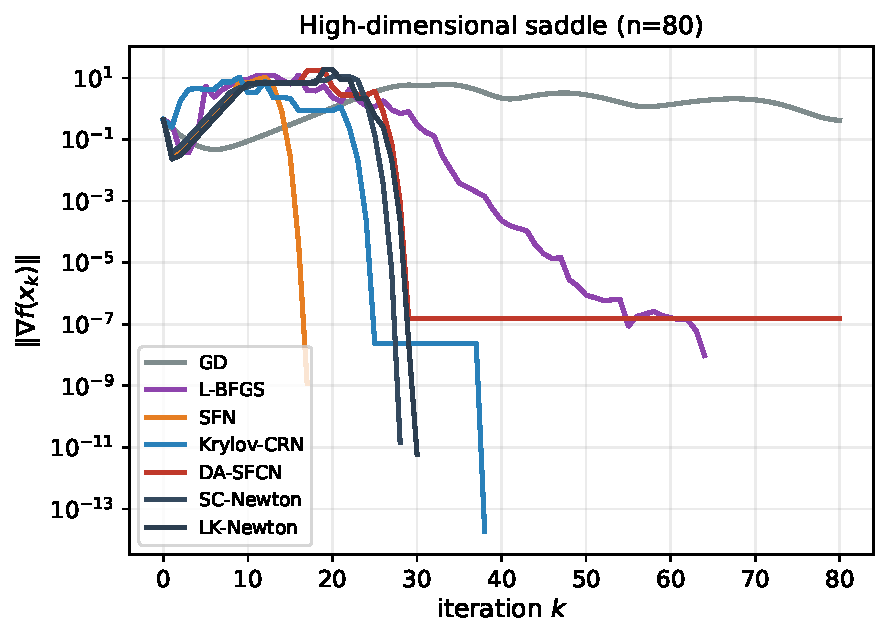
\includegraphics[width=0.48\textwidth]{fig_saddle_highdim.pdf}
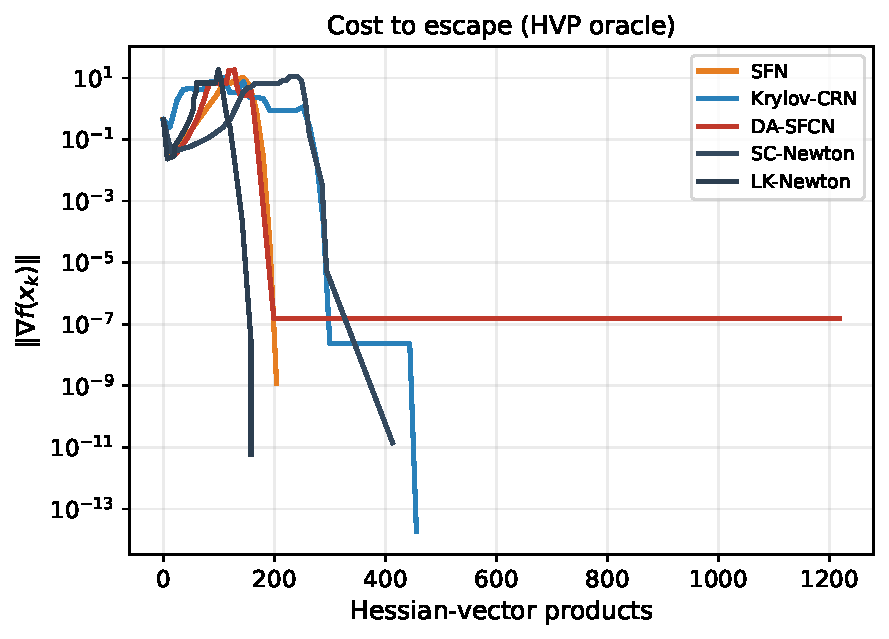
\includegraphics[width=0.48\textwidth]{fig_saddle_hvp.pdf}
\caption{\textenglish{LK-Newton} على السرج $n=80$: تكرارات (يسار) وجداءات (يمين).}
\end{figure}
\begin{figure}[h]
\centering
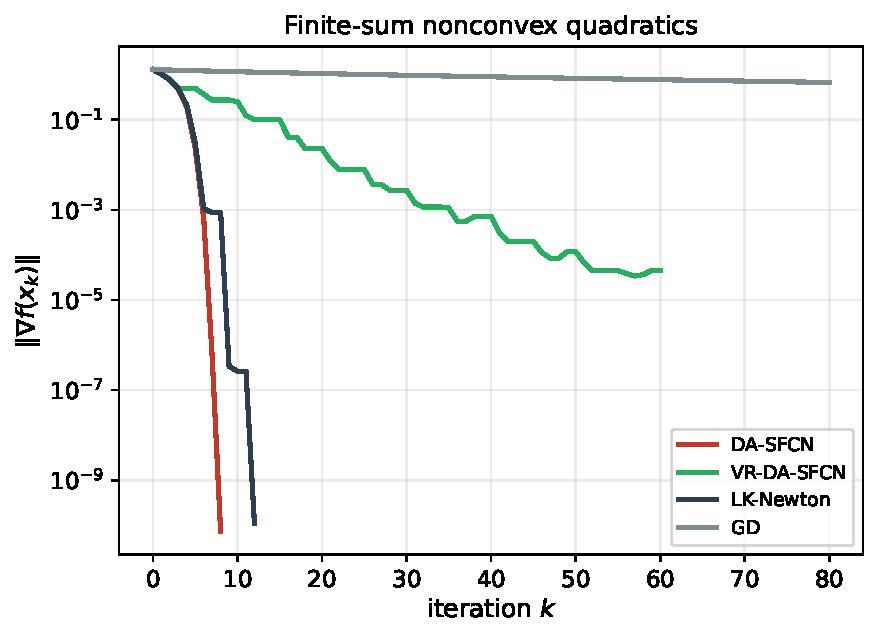
\includegraphics[width=0.48\textwidth]{fig_vr.pdf}
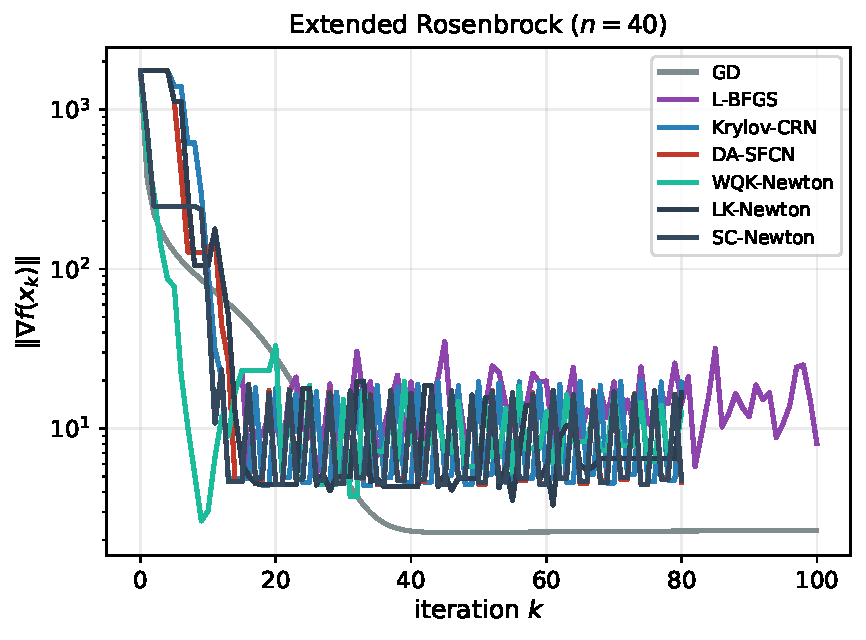
\includegraphics[width=0.48\textwidth]{fig_rosenbrock.pdf}
\caption{مجموع منتهٍ من التربيعيات وروزنبروك الممدَّد.}
\end{figure}

الرقم الأبرز: 158 جداءً مقابل 1219 مع تدرّج ختامي \emph{أفضل}. الكسل ليس
حيلة بل تخصيص أفضل للجبر الخطي بعد أن يلتقط المخطَّط البئر السالب.

\section{الخاتمة}
\textenglish{LK-Newton} الأرخص في تعقيد الأوراكل متى تغيّر المشهد ببطء نسبة
إلى $\tau$. ومع $m_k$ اللوغاريتمي نحصل على تكيّف مزدوج: عرض متكيف وإعادة
استخدام متكيفة.

\begin{english}
\begin{thebibliography}{9}
\bibitem{doikov2023} Doikov et al. Lazy Hessians. \textit{ICML}, 2023.
\bibitem{cartis2011} Cartis et al. \textit{Math.\ Program.}, 2011.
\bibitem{jiang2024} Jiang et al. \textit{AISTATS}, 2024.
\end{thebibliography}
\end{english}
\end{document}
